\documentclass[UTF8]{ctexart}
\usepackage{graphicx}
\usepackage{float}
\usepackage{geometry}
\usepackage{amsmath}
\usepackage{fancyhdr}
\usepackage{multirow}
\usepackage{multicol}
\usepackage{lastpage}
\usepackage{booktabs}
\geometry{left=2.54cm,right=2.54cm,top=3.18cm,bottom=3.18cm}%页边距
\pagestyle{fancy}
\lhead{
\includegraphics[scale=1]{sjtu-logo-red.pdf}}  
\rhead{项目标题} 
\cfoot{第 \thepage\ 页\ 共 \pageref{LastPage} 页} 

\begin{document}

\begin{titlepage}
    \begin{center}
        
\includegraphics[width=0.8\textwidth]{sjtu-name-blue.pdf}\\[1cm]
        \textsc{\Huge \bfseries 课程报告}\\[1.5cm]
        
\includegraphics[width=0.3\textwidth]{sjtu-badge-blue.pdf}\\[0.5cm]    

        \Huge \bfseries{基于深度学习的手术器械分割}\\[1cm]
        \Large \bfseries{518021910971 裴奕博}
    \end{center}
\end{titlepage}
\tableofcontents
\newpage
%正文

\section{项目简介}

\subsection{项目背景}
如今,医疗机器人已经在外科手术中有了广泛的应用,并且正朝着更高程度的精细化和自主化的方向发展。在机器人辅助手术的一个关键部分涉及到手术器械的跟踪和姿态的确定。由于手术过程中,图像受到光照、阴影、反射的影响,从图像中分割出手术器械是一大挑战。基于深度学习的方法在这样的图像分割中已经取得了不错的效果,因此本项目通过深度学习的方法,试图分割手术过程图像中的手术器械。

\subsection{项目流程}
本项目的流程如下:
\begin{figure}[H]
    \centering  %图片全局居中
    
\includegraphics[width=0.8\textwidth]{figure/workflow.png}
    \caption{项目工作流程图}
\end{figure}
整个流程和一般深度学习项目的流程相同,比较简单。
\subsection{项目任务}
本项目通过训练神经网络,实现对"binary","parts"和"instruments"三类问题在一定程度上的解决。其中,"binary"需要输出一张二值图像,仅代表器械与非器械。"parts"则需要表明其中一种器械主要器械的各个部分。"instruments"类则将对不同种类的手术器械进行分割。

\subsection{所用数据集}
选用了MICCAI endovis2017数据集,包括从instrument\_dataset\_1至7的共1800个样本。
原图像为24位色深的1920*1080的彩色png图像,ground truth为256个灰度级的1920*1080的黑白图像,不同的灰度代表不同的器械类别。

\subsection{文件结构与功能}
\begin{itemize}
    \item raw\_data文件夹:存放手术器械图像和ground truth的原始数据。
    \item cropped\_train文件夹:存放经过裁剪、重采样和灰度化预处理后的数据。
    \item runs文件夹:存放模型训练过程中产生的所有数据,包括模型结构、参数和训练记录log。
    \item prepare\_data.py文件:实现数据的预处理。
    \item prepare\_train\_val.py文件:规定用于训练和评估的数据集。
    \item dataset.py文件:定义Pytorch dataset和相关的图像和标签读取函数。
    \item loss.py文件:定义损失函数。
    \item validation.py文件:实现模型的评价指标的计算。
    \item train.py文件:模型训练的主程序。
    \item utils.py文件:定义其他所需的子模块。
    \item train.sh:训练脚本。
    \item result.json:存放训练的原始结果。
    \item json\_to\_csv.py:处理产生的原始数据并将其转换为csv格式。
    \item result.csv:最终生成的评估结果表格。
\end{itemize}


\section{实现方法}
\subsection{数据预处理}
\subsubsection{图像的下采样}
由于原图和ground truth均为1920*1080,单张图像素点很多,如果直接输入神经网络会导致参数量过多且运行速度缓慢,因此在数据预处理时通过下采样将输入数据转化为640*512
\subsubsection{标签的分类}
根据用户所要解决的问题,需要将标签进行对应的分类,可以看到在cropped\_train文件夹下分别对应三种问题类型的mask。在数据预处理中即将其分开。对原数据集中的Left ground truth进行二值化后即可得到binary masks,将Left ground truth重新映射到(0,255)即可得到parts masks,而对其他文件夹的文件进行总和即可得到instruments masks。
\subsubsection{数据增强}
本次数据集样本量较少,为使得神经网络训练达到更好的效果,需要进行数据增强。本次项目采用了padding,随机裁切,水平垂直翻转,正则化等数据增强方法,有效扩充了数据量。

\subsection{网络结构实现}
\subsubsection{基于UNet的方法}

根据\cite{shvets2018automatic}中提供的方法,复现了论文中的UNet,UNet-11,UNet-16和LinkNet-34四种方法。这四个网络均为基于UNet的全卷积网络。
\begin{itemize}
    \item UNet是一种经典的网络,前半部分通过CNN编码器提取特征,逐步下采样,后半部分通过反卷积的方式进行上采样,并增加了跳跃的连接以减慢梯度的下降,使网络能够更深。最后输出与原图大小一致的预测值,可以直接与label进行比较计算loss,是图像分割中常见的基本网络。
    \item UNet-11和UNet-16是对UNet的改进,两者均采用了VGGNet作为encoder,UNet11和UNet15也是根据两者使用的encoder为VGG-11和VGG-16命名。
    \begin{figure}[H]
        \centering  %图片全局居中
        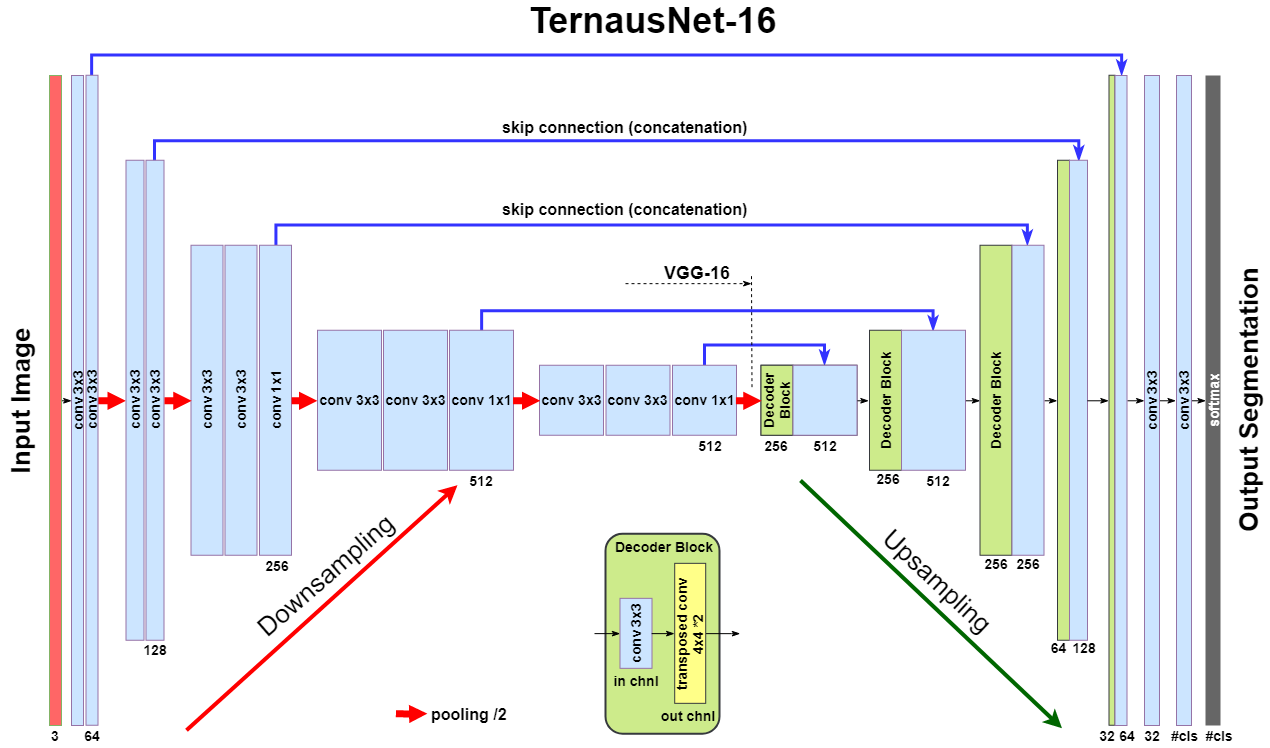
\includegraphics[width=0.8\textwidth]{figure/TernausNet.png}
        \caption{TernausNet结构图}
    \end{figure}
    \item LinkNet-34是另一种对UNet的改进方法,采用了ResNet-34作为encoder。此外在decoder block上也有了改进:添加了batch normalization和1*1的卷积。
    \begin{figure}[H]
        \centering  %图片全局居中
        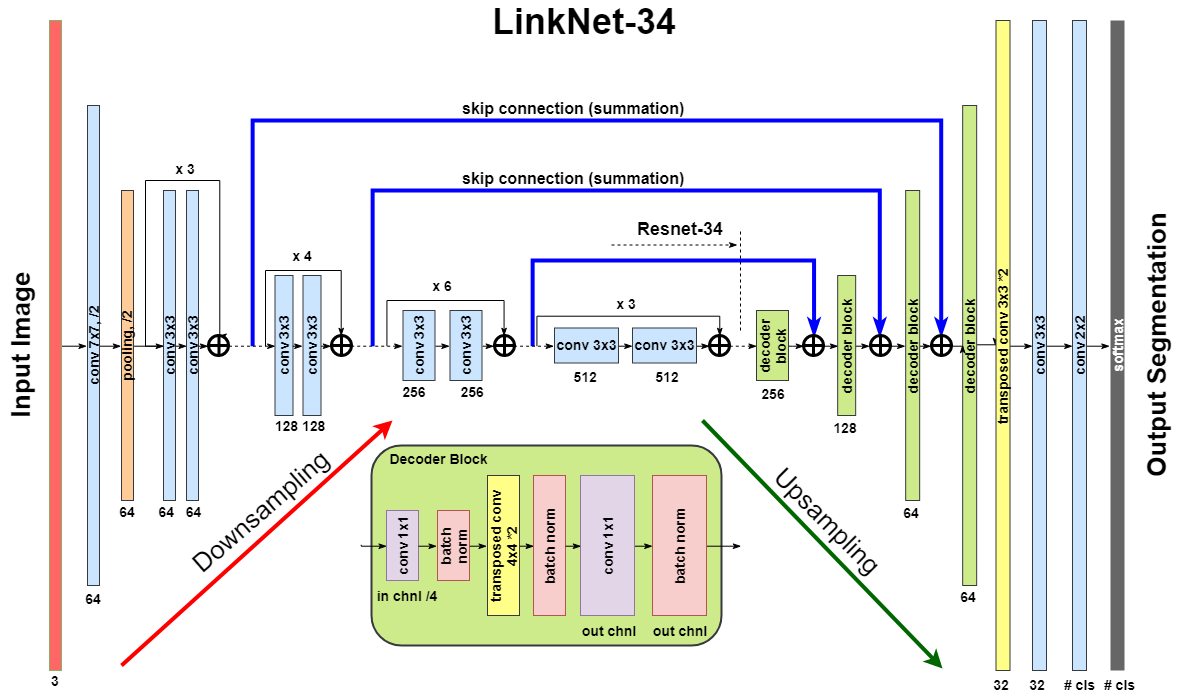
\includegraphics[width=0.8\textwidth]{figure/LinkNet34.png}
        \caption{LinkNet结构图}
    \end{figure}
\end{itemize}

\subsubsection{基于TDSNet的多任务网络}
此外,由于以上几种网络对instrument类问题的分割效果并不好,因此考虑到各类问题之间的相互关联关系,设计了基于TDSNet\cite{ren2019task}
的多任务网络。

\begin{figure}[H]
    \centering  %图片全局居中
    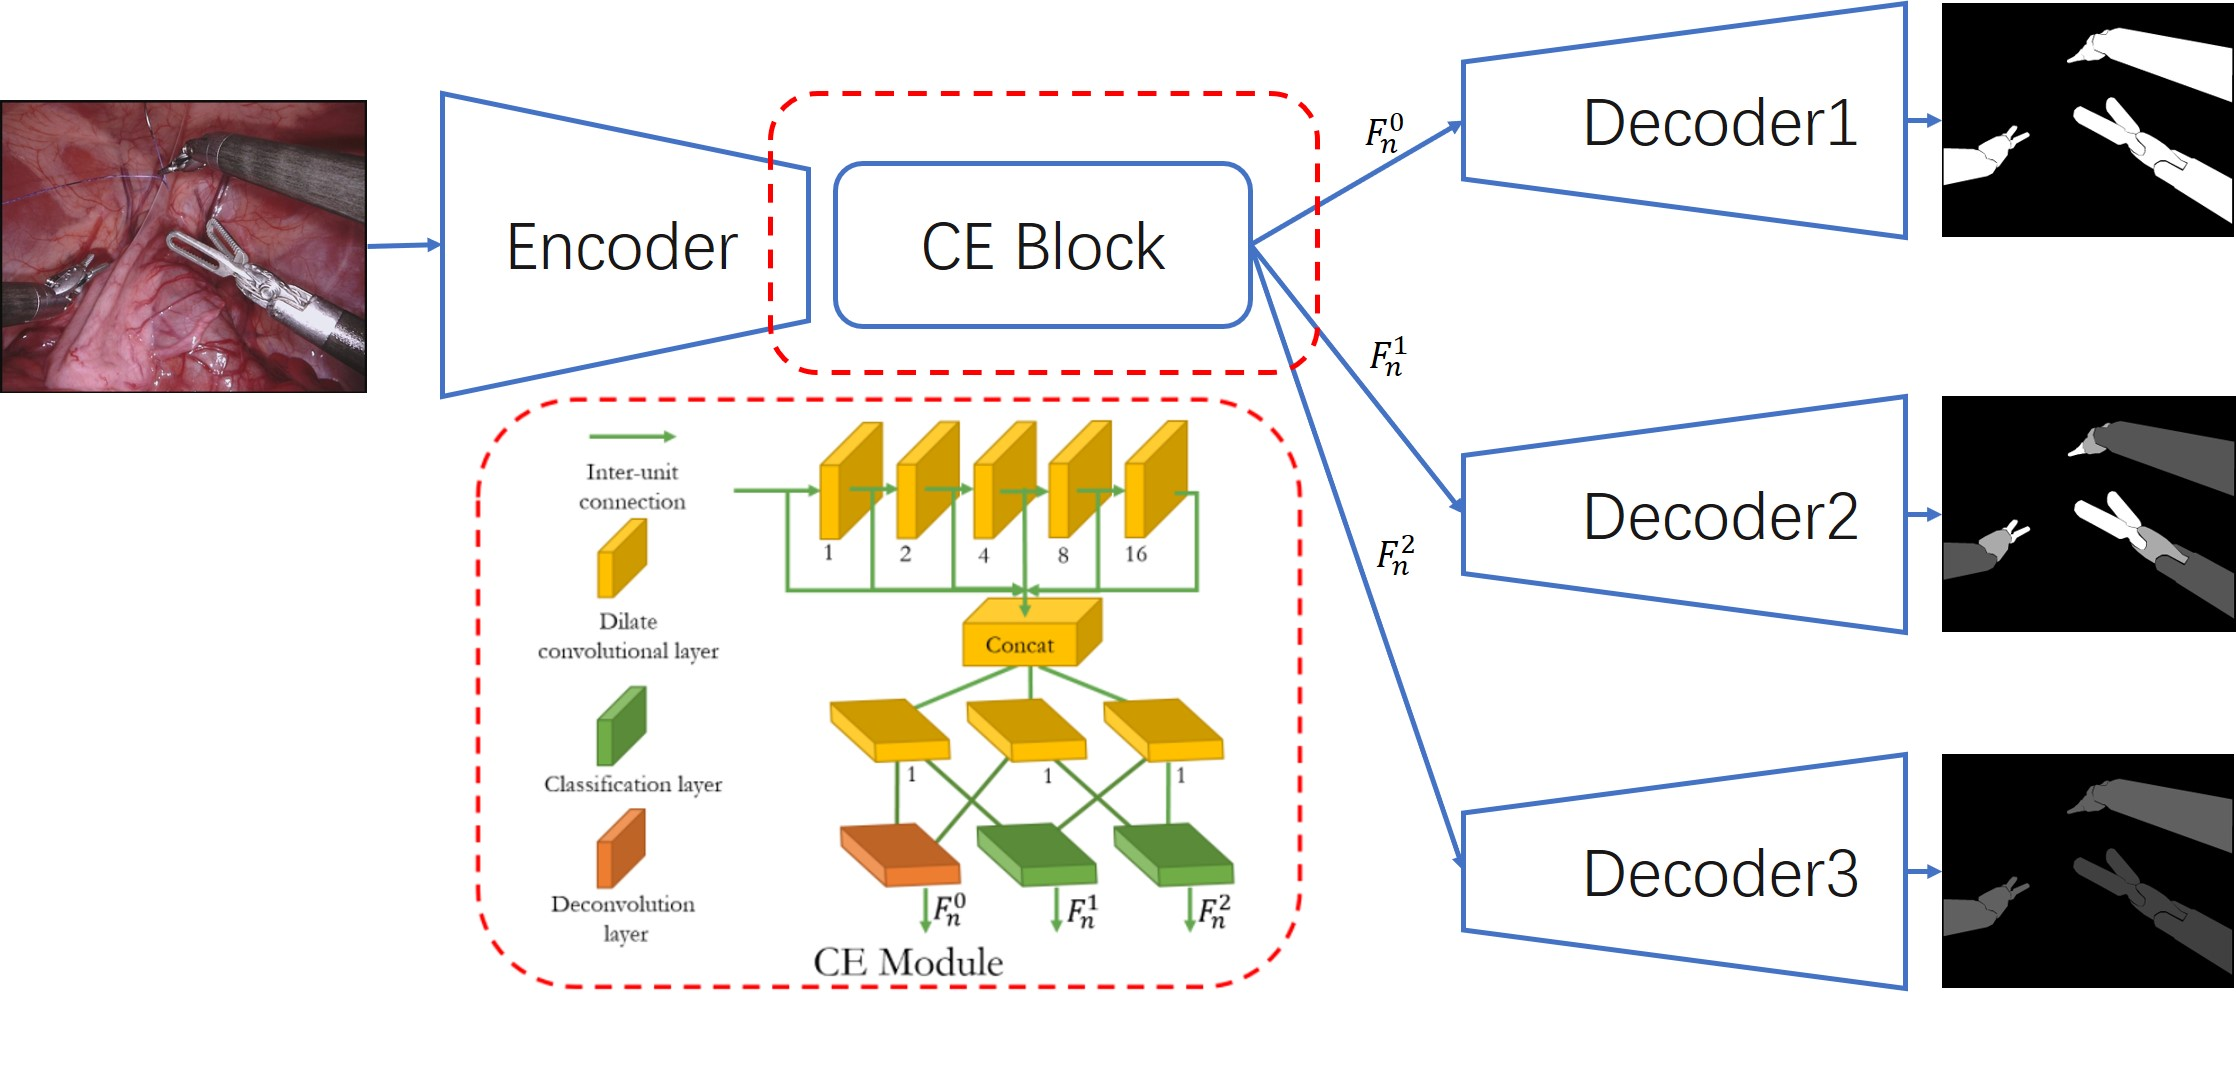
\includegraphics[width=0.8\textwidth]{figure/TDSNet.jpg}
    \caption{TDSNet结构图}
\end{figure}
TDSNet的要点在于在encoder和decoder之间插入了一个CE Block,在这个CE Block中依次使用了不同步长的dilate convolution以整合不同大小的特征。随后将CE Block的输出$F_n^0,F_n^1,F_n^2$输入三个decoder,并对应三种不同的分类任务。这样将三个不同的任务共用一个encoder,在理论上可以避免模型参数过多,并且在重点进行其中一个任务的分割时,可以有效利用到其他两个任务ground truth中所包含的信息,同时也提升了模型的运行速度。

\subsection{训练参数的选取}
\begin{itemize}
    \item 选用$L=H-k\log J$作为损失函数,其中H为交叉熵(cross entropy),k为常数(实际训练时取0.3),J为dice score,可以表示为
    $$J=\frac{1}{n}\sum_{i=1}^n(\frac{y_i\hat{y}_i}{y_i+\hat{y}_i-y_i\hat{y}_i})$$
    在使用TDSNet时,损失函数为三者的加权和,实际使用时binary,parts,instruments三者的权重分别为0.4,0.3,0.3
    \item 选用的优化器为Adam,batch size取16(TDSNet由于参数量大,取8)。
    \item 学习率采用阶梯式,即前10个epoch采用1e-4使其更快收敛,后十个epoch采用1e-5。
    \item 将数据集分为[1, 3],[2, 5],[4, 8] [6, 7]四个fold,每次取其中一组作为valid set其余作为训练集,进行交叉验证算法。
\end{itemize}


\section{结果评估}
\subsection{评价指标的选取}
由于模型的输出和ground truth均为分割后的图像,因此评价指标的选取就比较简单,采用了图像分割中常用的iou和dice作为评价指标。定义预测为阳性的区域为A,ground truth中阳性区域为B,则两者的计算公式如下:

\begin{equation}
    IoU=\frac{|A\cap B|}{|A\cup B|}=\frac{|A\cap B|}{|A|+|B|-|A\cup B|}
\end{equation}

\begin{equation}
    Dice=\frac{2|A\cap B|}{|A|+|B|}
\end{equation}
此外,也同时输出valid loss作为对照

\subsection{各方法评价指标对比}
输出所用网络针对于各类问题的评价指标数据(TDSNet的指标为单次运行时分出的数据)。输出表格如下:

% Table generated by Excel2LaTeX from sheet 'result'
\begin{table}[H]
    \centering
    \caption{各模型评价指标对比}
      \begin{tabular}{clrrr}
        \toprule
      \multicolumn{1}{l}{model} & problem-type & \multicolumn{1}{l}{valid\_loss} & \multicolumn{1}{l}{iou} & \multicolumn{1}{l}{dice} \\
        \midrule
      \multirow{3}[0]{*}{LinkNet34} & binary & 0.291619 & 0.83452 & 0.90916 \\
            & instruments & 39.55267 & 0.169484 & 0.254484 \\
            & parts & 1.482577 & 0.752365 & 0.849873 \\
            \midrule
      \multirow{3}[0]{*}{TDSNet} & binary & 15.81483 & 0.440223 & 0.609769 \\
            & parts & 15.81483 & 0.436848 & 0.590687 \\
            & instruments & 15.81483 & 0.094368 & 0.159233 \\
            \midrule
      \multirow{3}[0]{*}{UNet} & binary & 0.372041 & 0.733065 & 0.845729 \\
            & instruments & 41.29976 & 0.113255 & 0.18736 \\
            & parts & 2.061818 & 0.57118 & 0.70922 \\
            \midrule
      \multirow{3}[0]{*}{UNet11} & binary & 0.264989 & 0.855534 & 0.921626 \\
            & instruments & 40.18801 & 0.163311 & 0.252311 \\
            & parts & 1.347551 & 0.739667 & 0.841694 \\
            \midrule
      \multirow{3}[0]{*}{UNet16} & binary & 0.252788 & 0.864523 & 0.927097 \\
            & instruments & 40.19258 & 0.189746 & 0.277829 \\
            & parts & 1.229443 & 0.776812 & 0.869413 \\
            \bottomrule
      \end{tabular}%
    \label{tab:addlabel}%
  \end{table}%
可以看到以下几点:
\begin{itemize}
    \item 最基本的UNet在binary问题上有不错的表现,但在其他问题上与改进后的其他网络有明显差距。
    \item 总体来说,对于binary和parts的分割都取得了不错的效果。UNet11,UNet16和LinkNet34均达到了较高的iou和dice。其中UNet16的效果最好,但网络结构也最为复杂,参数量最大,LinkNet则在参数量减少的同时达到了不错的效果。
    \item TDSNet表现不佳,在三个问题上均与其他网络有很大的差距。
\end{itemize}

  
\subsection{可视化结果对比}

\begin{figure}[H]
    \centering  %图片全局居中
    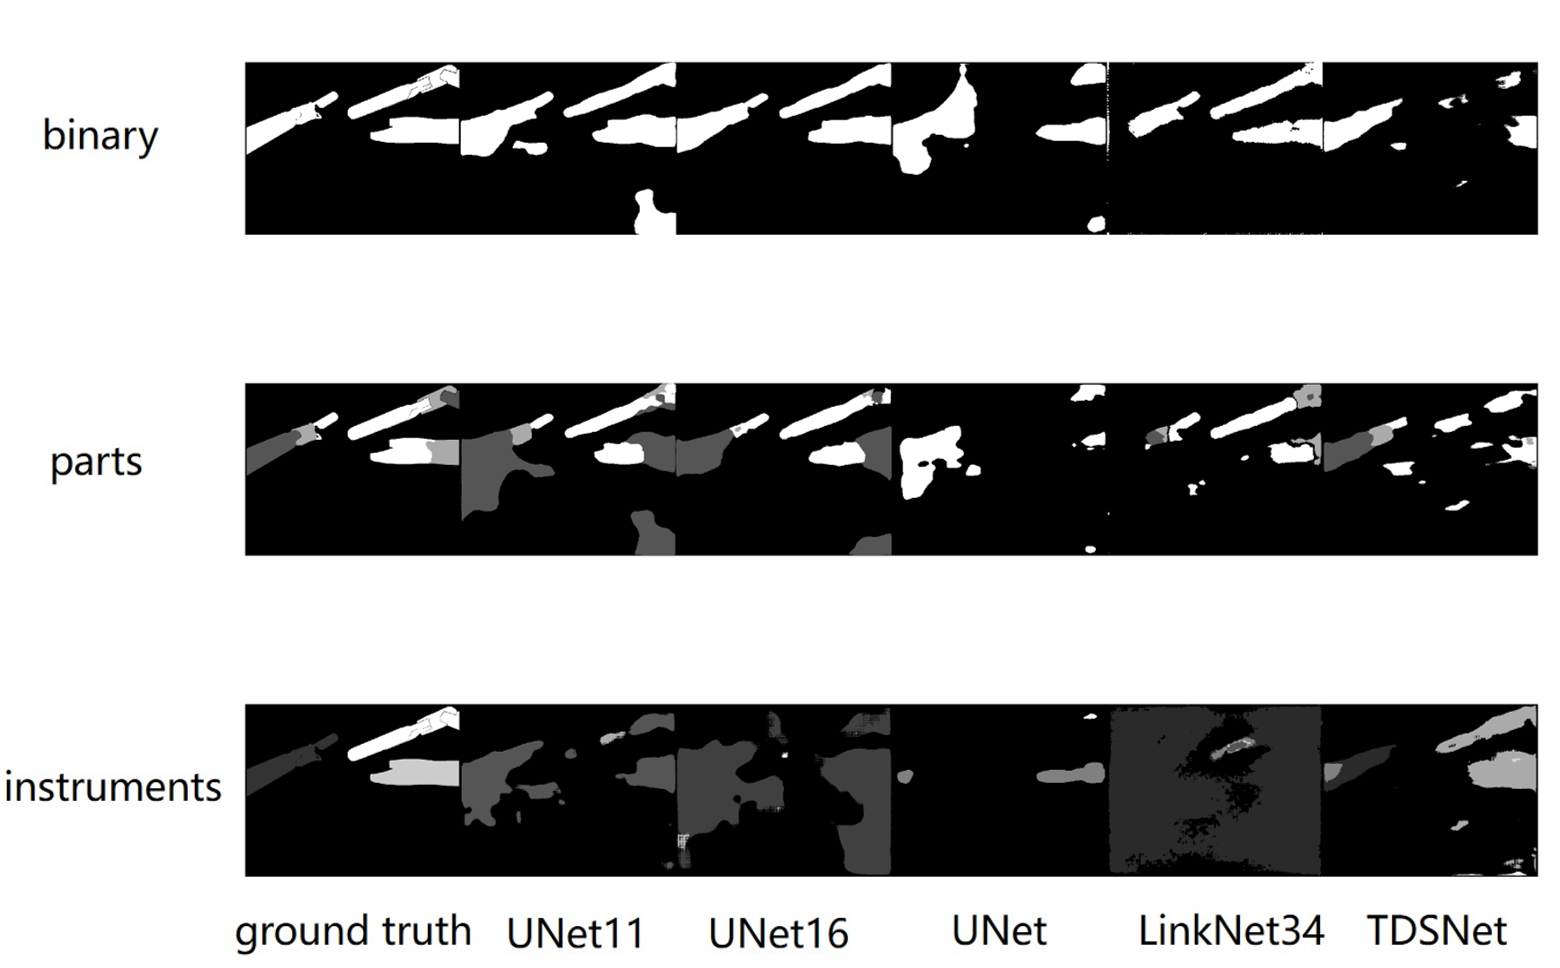
\includegraphics[width=0.8\textwidth]{figure/visualize.png}
    \caption{可视化结果对比图}
\end{figure}

\begin{itemize}
    \item 可以看到,总体结果与iou和dice显示的指标一致,UNet11和UNet16的表现是最好的。
    \item 还可以注意到,在instruments类的分割中,TDSNet其实表现的没有评价指标显示的那么糟糕,基本分割出了边缘,评价指标低的原因是因为大面积的分错类,而这一现状在其他网络中多多少少也存在。
\end{itemize}

\subsection{结果分析}
可以看到,在binary问题和parts问题上,许多方法都达到了不错的效果,但对于instruments则效果不佳。产生这一结果的原因可能是数据集中各类样本的不平衡。查看数据集就会发现,部分手术器械的类别在数据集中很少出现,甚至在某些fold中整类器械一次都没有出现过,这对神经网络进行判断产生了很大的困难。与之对应的时,在最终输出的结果中,出现了大面积的分错类的现象,而非传统中更容易出现的分割边缘上的错误。这也解释了为什么神经网络在parts问题上表现良好而在instruments问题上发挥不佳。

TDSNet在各类问题上表现不佳。推测原因可能有以下几点:
\begin{itemize}
    \item 首先是模型的参数过多。在Shvets等人\cite{shvets2018automatic}的工作
    中,需要解决的问题是一个图像分割问题和两个one-hot的分类问题,而在本项目中,需要输出的是三个分割好的图像,在网络的后半部分需要三个结构相同的decoder,因此相比原文中网络结构更为复杂,更难训练。
    \item 其次是在当前版本的TDSNet中,我将binary,parts和instruments放在了同等重要的地位,而事实上,binary是其余两者的基础,parts和instruments可以看作binary问题的进一步延伸。可能这样的差异会使网络的效果下降。
    \item 最后是可能由于时间有限,模型的训练过程和各个超参数都未能调整到更佳,在不改变网络结构的情况下通过改变超参数也可能会达到更好的效果。
\end{itemize}


\section{项目总结与展望}
本次项目通过深度学习的方法完成了对手术器械的分割,在binary和parts任务上表现良好,但对于instuments任务表现欠佳,自己搭建的多任务网络也没有取得预期的效果,只能说是部分完成了预期目标,还有很多可以改进的空间。

尽管效果不尽如人意,但是在本次大作业中我还是收获很多。本次大作业是我第一次真正有机会独立完成有关深度学习的项目。在完成项目的时间里,我学习了一些关于深度学习的基本知识,Pytorch框架的使用和一个深度学习项目基本的组成部分,也完成了从原始数据集到模型训练验证的整个流程。根据老师给的参考资料上的思路,也自己搭建了一个基于TDSNet的神经网络。虽然可能因为一些细节的问题导致效果不佳,但是在完成项目的过程中我还是学到了很多,并且接触到了实际的科研问题,也算是对深度学习这个热门领域有了入门的了解。

最后模型实现的结果没能达到预期还是比较遗憾,但是个人在完成项目的过程中也收获了很多。最后感谢老师和助教在本次项目完成过程中给予我的帮助!

\bibliography{ref}
\bibliographystyle{ieeetr}

\end{document}
